\chapter{Tutorial Membuat Aplikasi dengan APEX}
Bagaimanasih Cara membuat Aplikasi menggunakan Apex

\section{Tutorial APEX}

\begin{enumerate}
\item Pertama, kita buat dahulu \textit{workspace} di website \url{https://apex.oracle.com/en/} 

\item Lalu, isi semua data dengan benar,kemudian login ke dalam workspace 
\begin{figure}[H]
\centering
\caption{Halaman Utama Workspace}
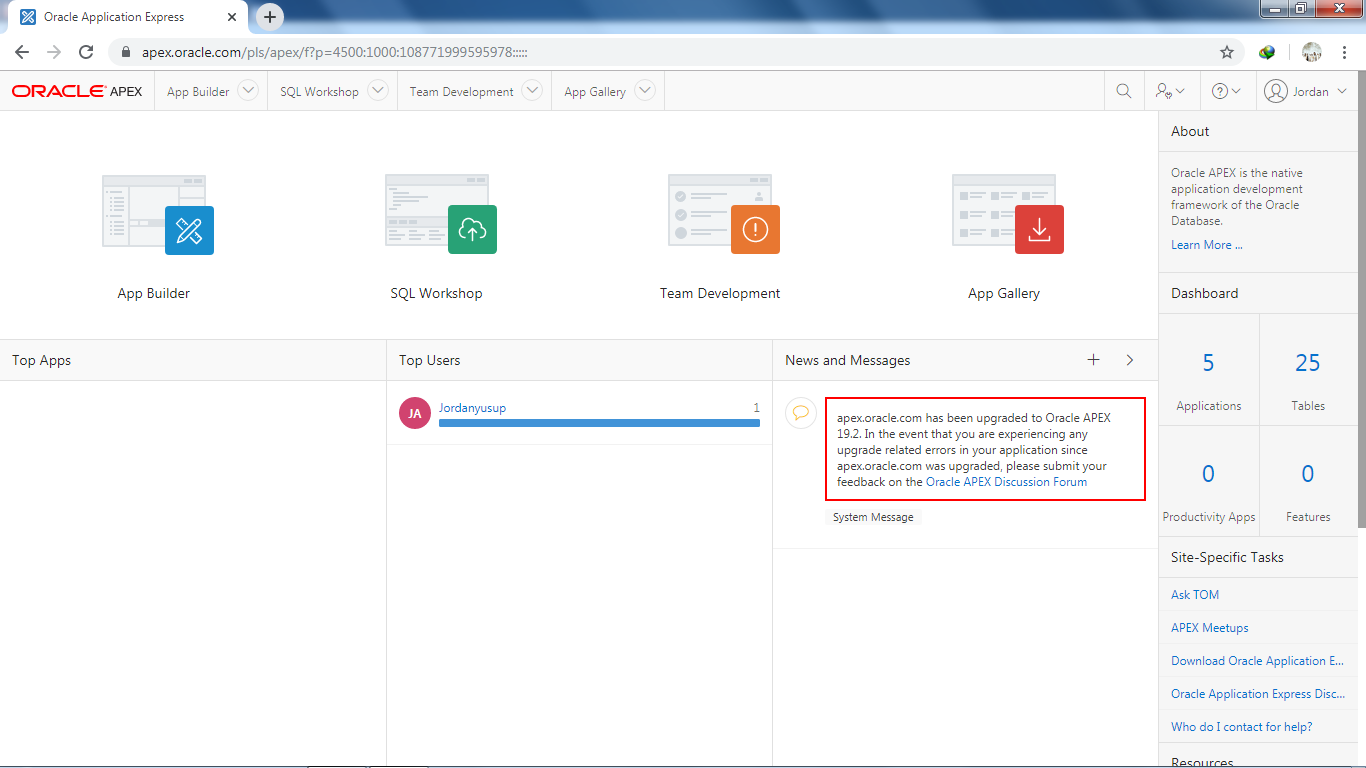
\includegraphics[width=1\textwidth]{figures/1.png}
\end{figure}

\item Setelah itu klik \textit{app builder} dan klik create  
\begin{figure}[H]
\centering
\caption{Halaman App Builder}
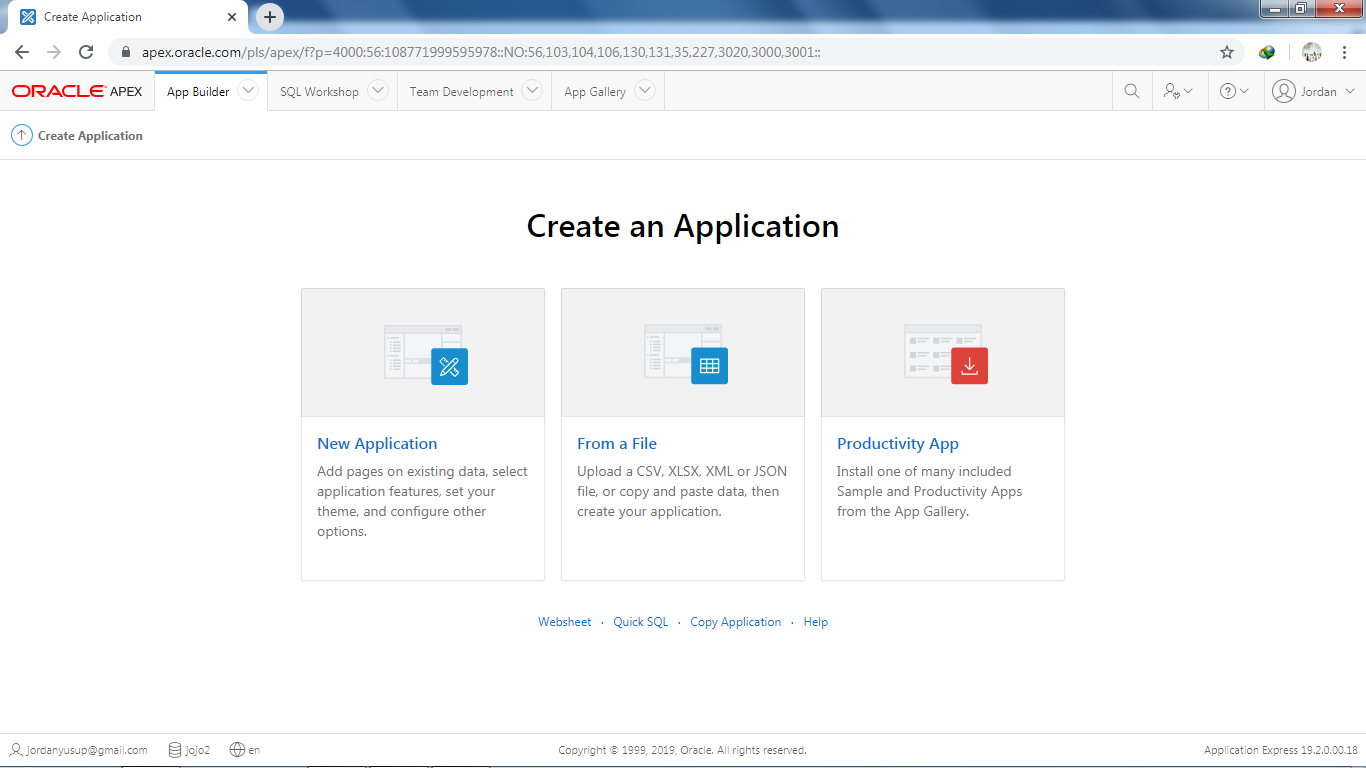
\includegraphics[width=1\textwidth]{figures/2.png}
\end{figure}

\item Selanjutnya, pilih From a File
\begin{figure}[H]
\centering
\caption{Halaman Upload File}
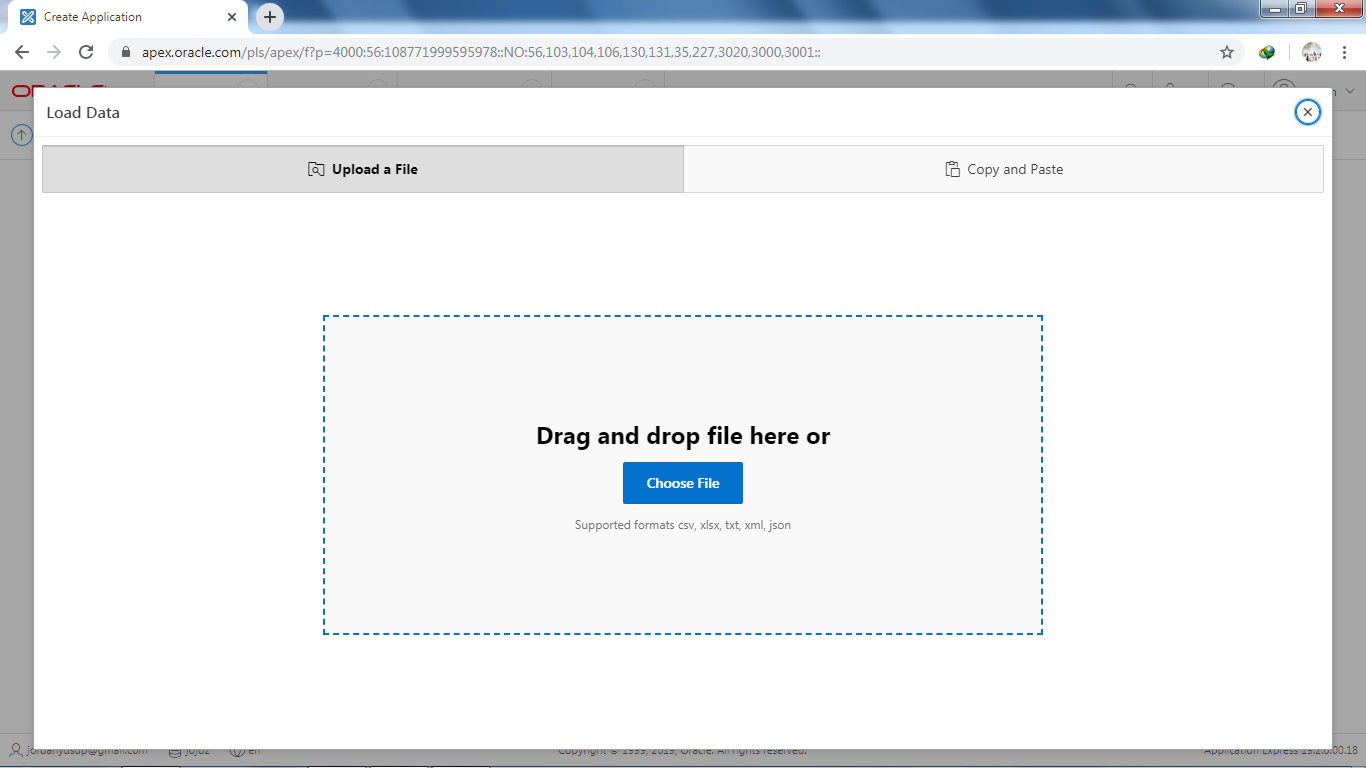
\includegraphics[width=1\textwidth]{figures/3.png}
\end{figure}

\item Setelah itu akan muncul window untuk memilih file xlsx atau csv
\begin{figure}[H]
\centering
\caption{Form Upload FIle}
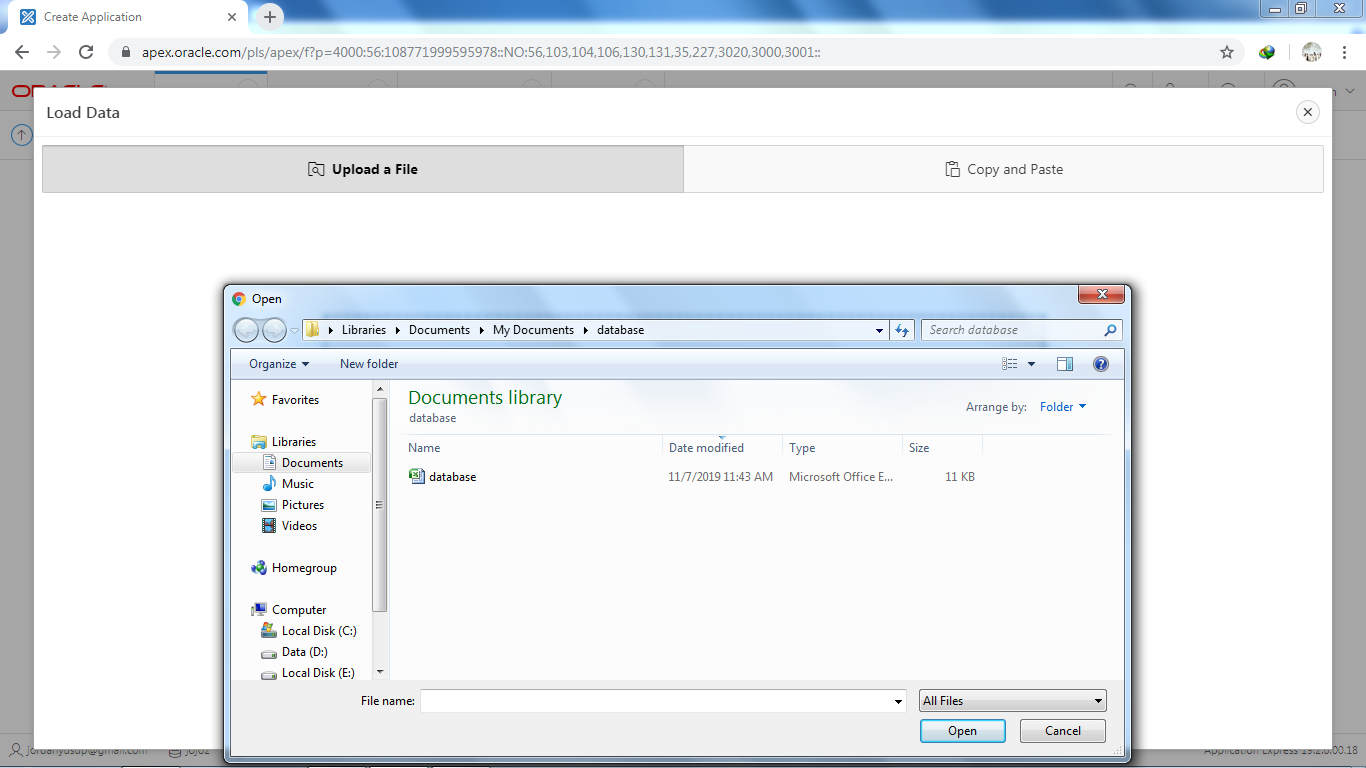
\includegraphics[width=1\textwidth]{figures/4.png}
\end{figure}

\item Kemudian pilih dan klik open
\begin{figure}[H]
\centering
\caption{Hasil Upload File}
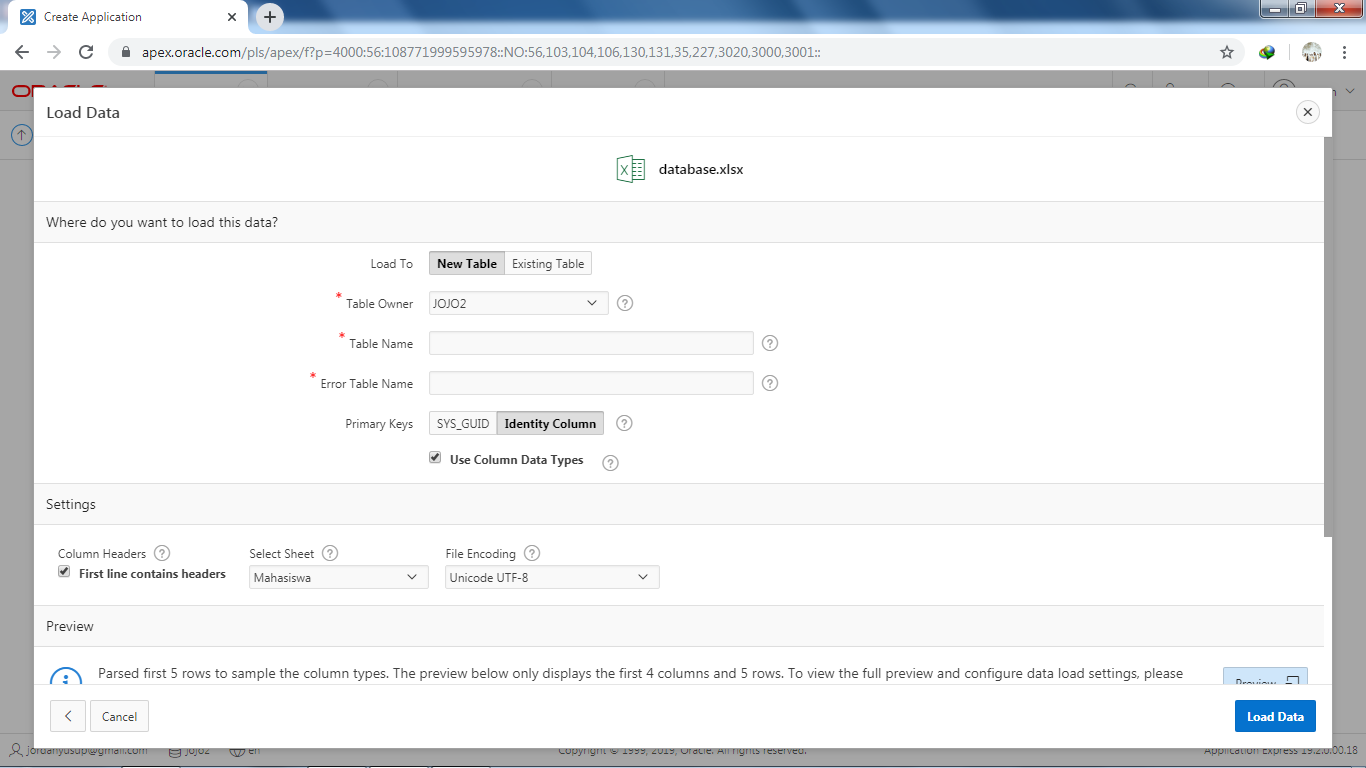
\includegraphics[width=1\textwidth]{figures/5.png}
\end{figure}

\item Setelah kita pilih selanjutnya kita masukkan nama tabelnya. Di bagian Field eror table name akan terisi otomatis
\begin{figure}[H]
\centering
\caption{Masukkan Table Name dan Error Table Name}
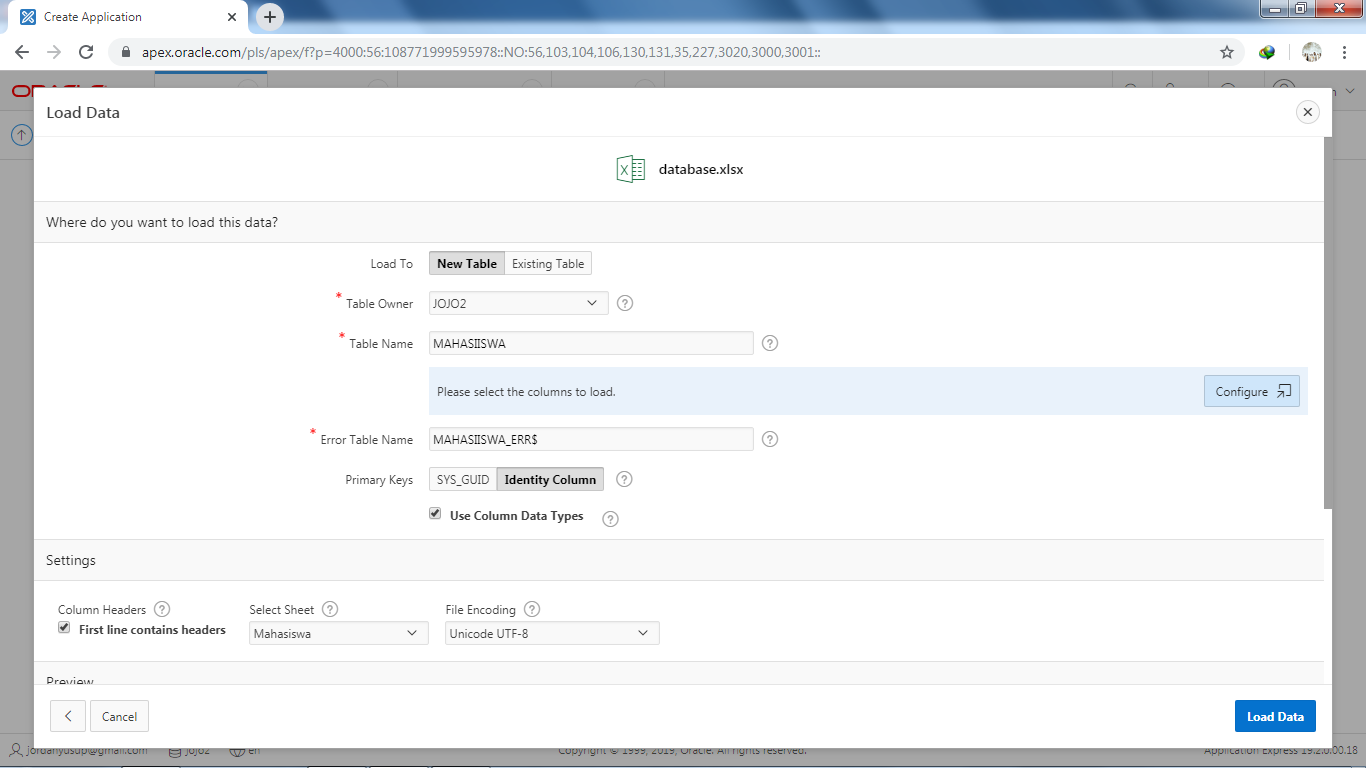
\includegraphics[width=1\textwidth]{figures/6.png}
\end{figure}

\item Pilih configure dan pastikan bahwa atribut sudah benar
\begin{figure}[H]
\centering
\caption{Configure Tabel}
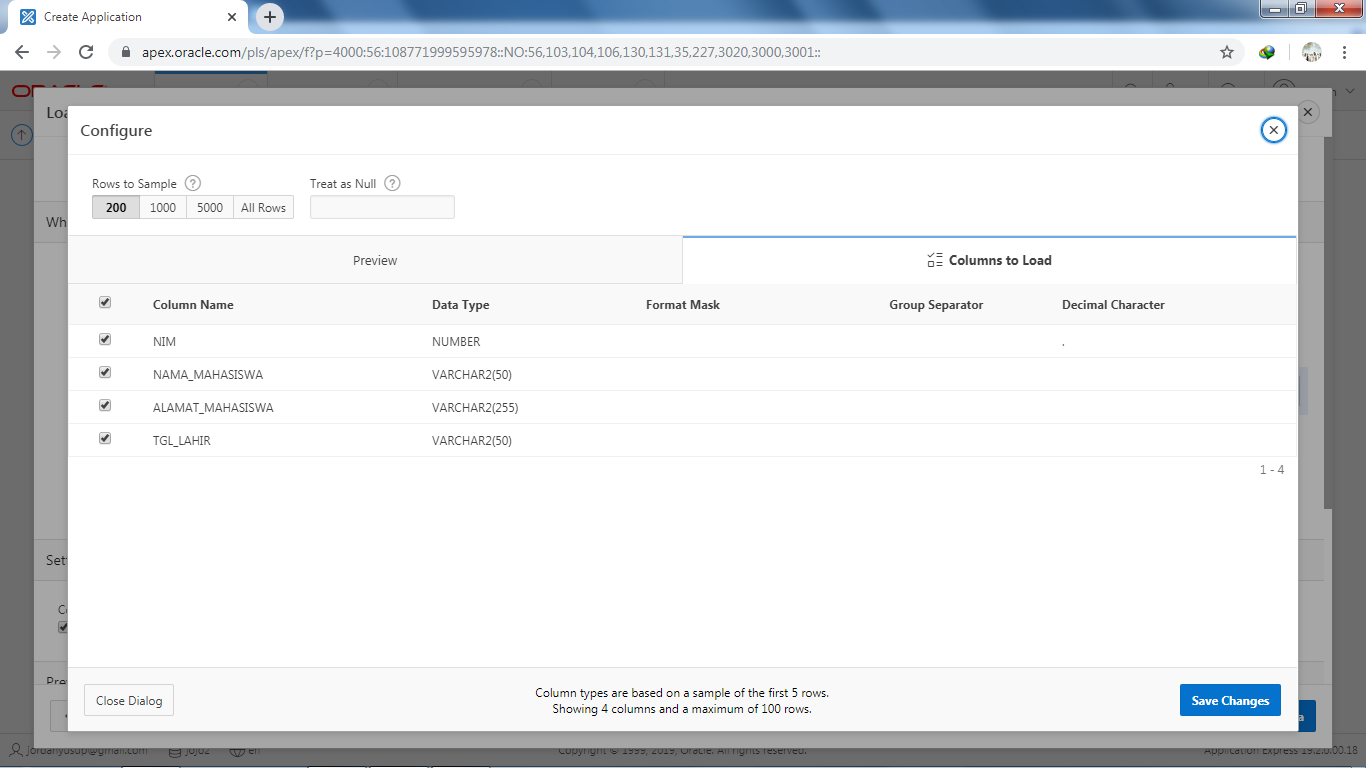
\includegraphics[width=1\textwidth]{figures/7.png}
\end{figure}

\item Selanjutnya klik save change untuk menyimpan tabel
\begin{figure}[H]
\centering
\caption{Selesai Save Change}
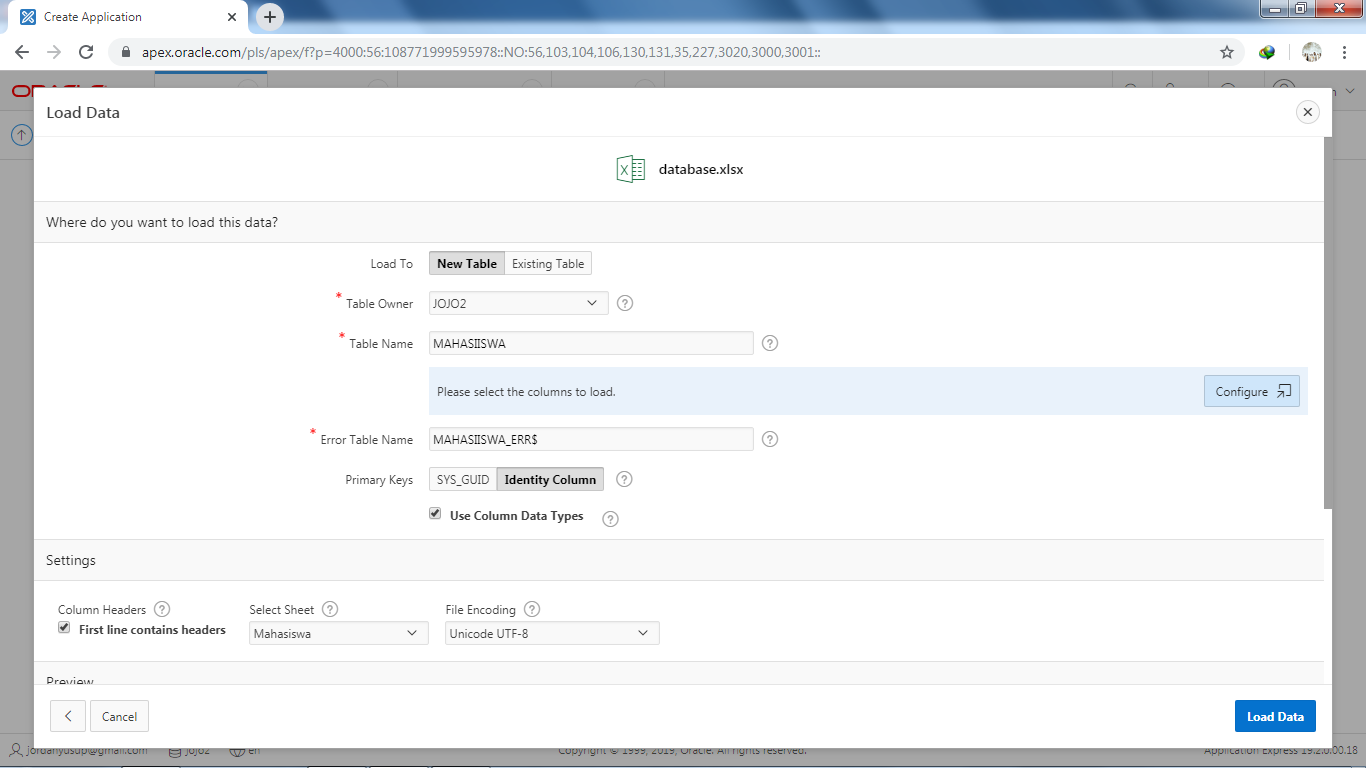
\includegraphics[width=1\textwidth]{figures/6.png}
\end{figure}

\item Kemudian klik load data
\begin{figure}[H]
\centering
\caption{Upload Selesai}
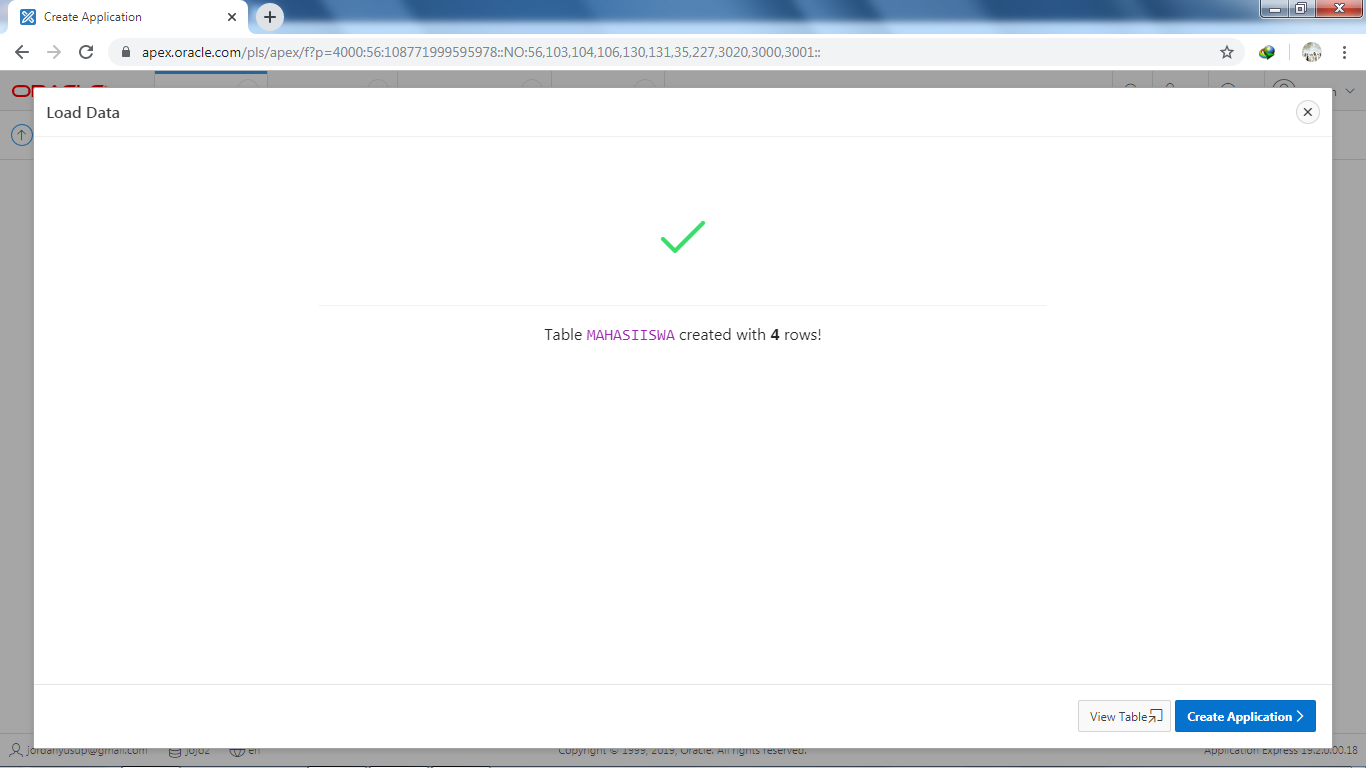
\includegraphics[width=1\textwidth]{figures/8.png}
\end{figure}

\item Lakukan ulang kembali dari langkah 3 sampai langkah 10 sesuai jumlah tabel yang digunakan

\item Selanjutnya buka tabel yang telah dibuat, Maka disana akan muncul kolom id yang dibuat otomatis oleh sistem karena tabel tidak ada primary key.

\item Pilih sql workshop lalu ke object browser
\begin{figure}[H]
\centering
\caption{SQL Workshop -> Object Browser}
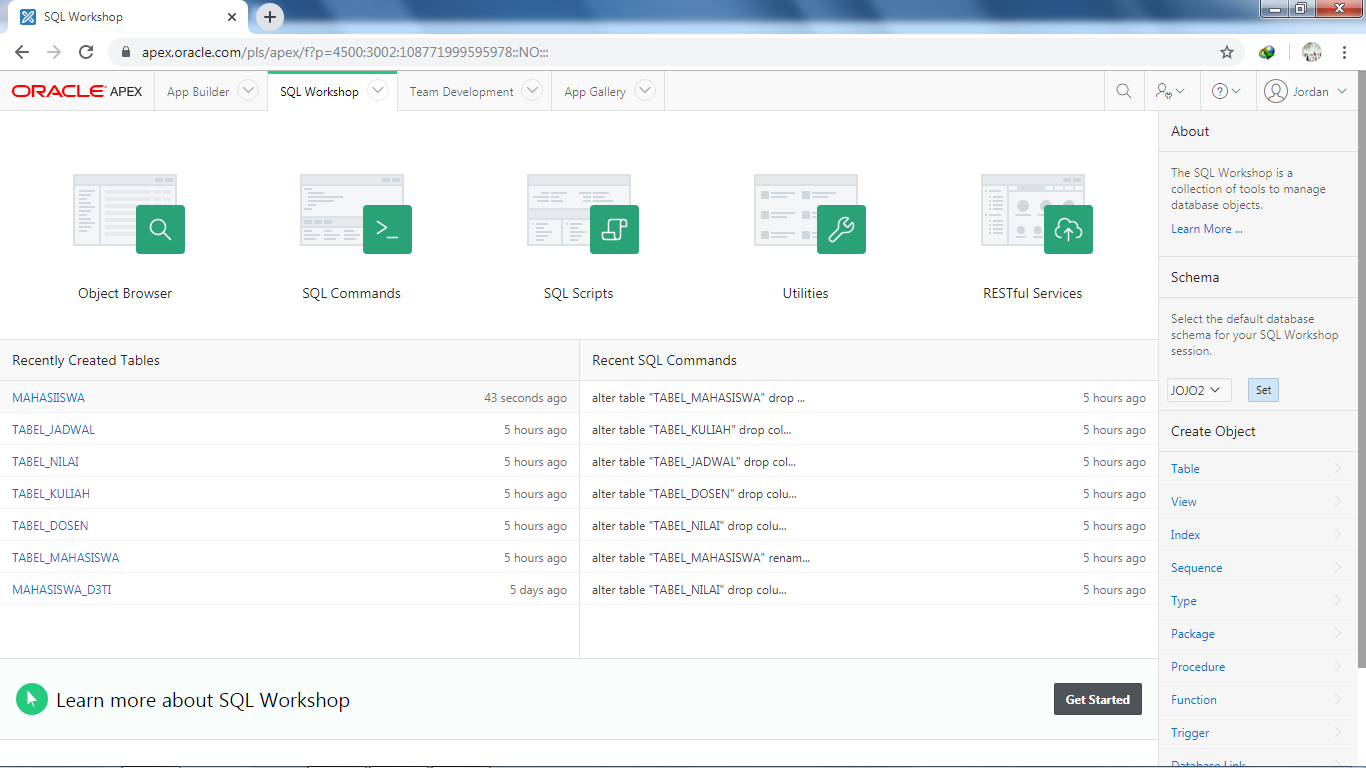
\includegraphics[width=1\textwidth]{figures/9.png}
\end{figure}

\item Selanjutnya kita klik tabel yang ingin kita hapus.
\begin{figure}[H]
\centering
\caption{Tabel Drop}
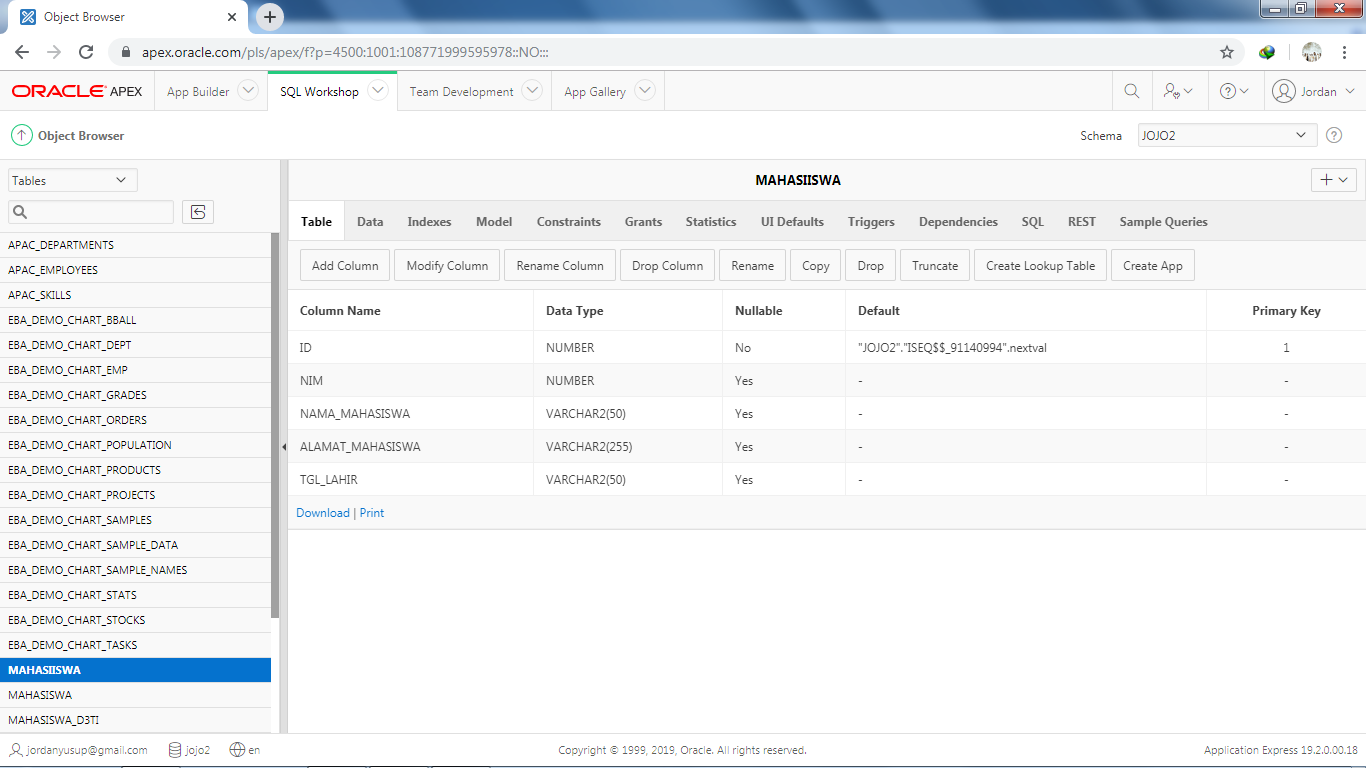
\includegraphics[width=1\textwidth]{figures/10.png}
\end{figure}

\item Klik Drop Column dan pilih kolom yang ingin di hapus. lalu klik drop lagi dan klik finish. Lakukan berulang kali agar tidak ada kolom id yang tersisa.

\item Selanjutnya menambahkan primary key kesetiap tabel yang telah kita buat.

\item Lalu kita ketikkan query seperti pada gambar
\begin{figure}[H]
\centering
\caption{Query Add Primary Key}
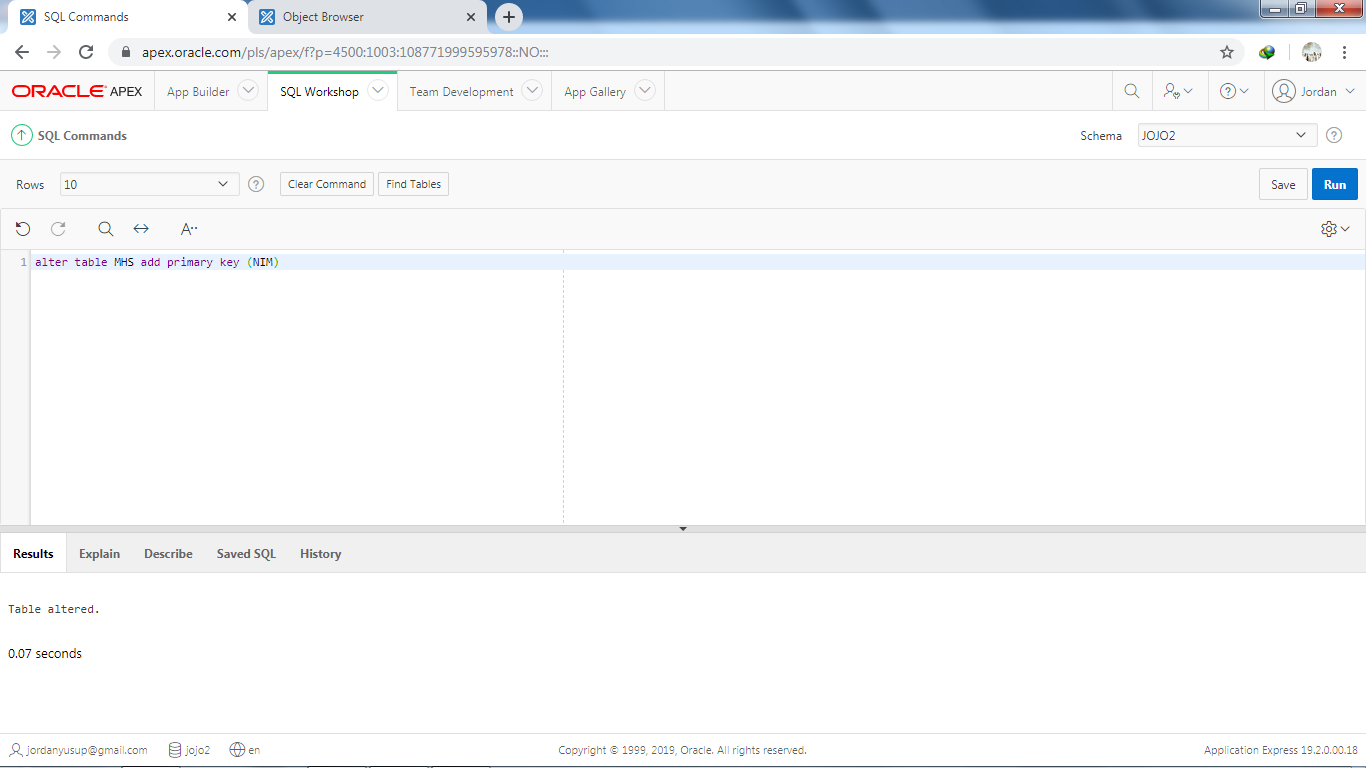
\includegraphics[width=1\textwidth]{figures/12.png}
\end{figure}

\item Kemudian pilih run, jika berhasil akan muncul pesan table altered.

\item Langkah selanjutnya adalah cara merelasikan dua tabel
\begin{figure}[H]
\centering
\caption{Query Add Foreign Key}
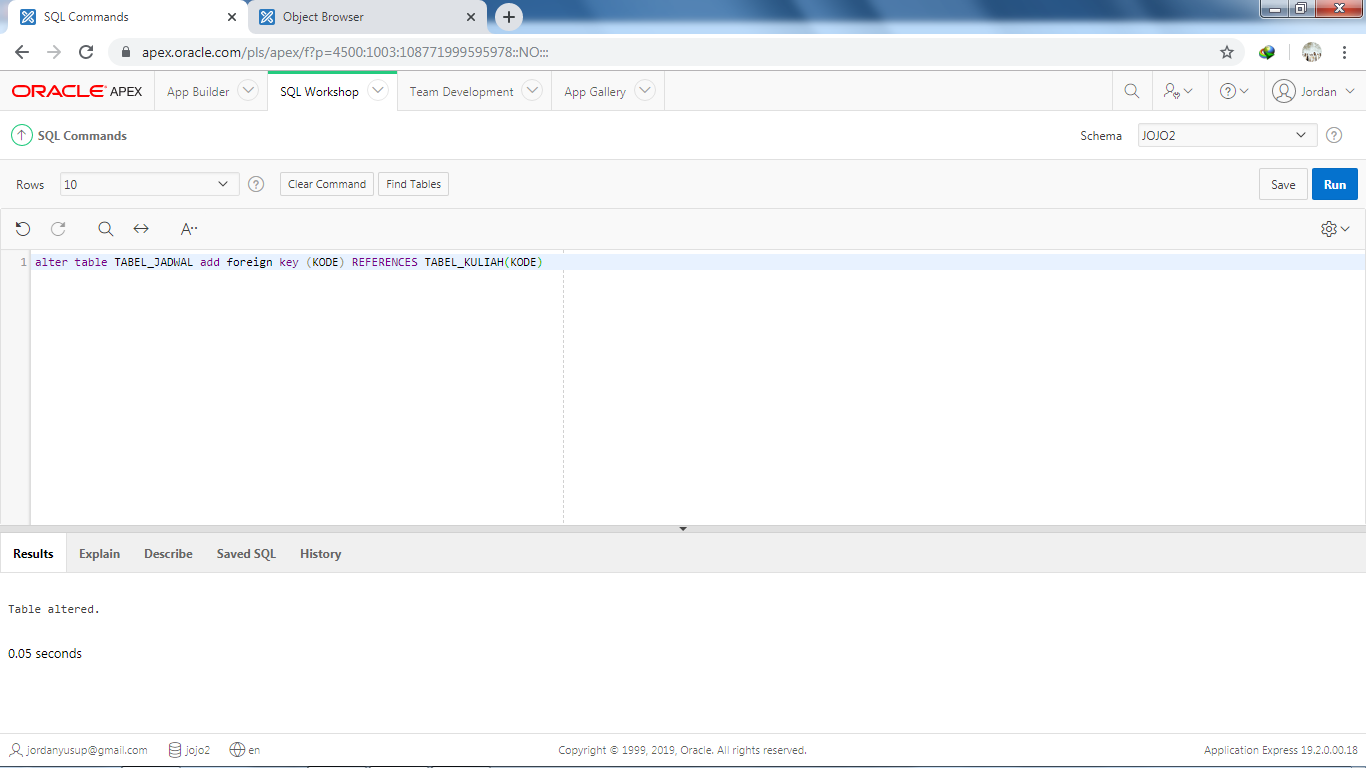
\includegraphics[width=1\textwidth]{figures/13.png}
\end{figure}

\item Selanjutnya pilih app builder kemudian klik create dan klik new application
\begin{figure}[H]
\centering
\caption{New Application}
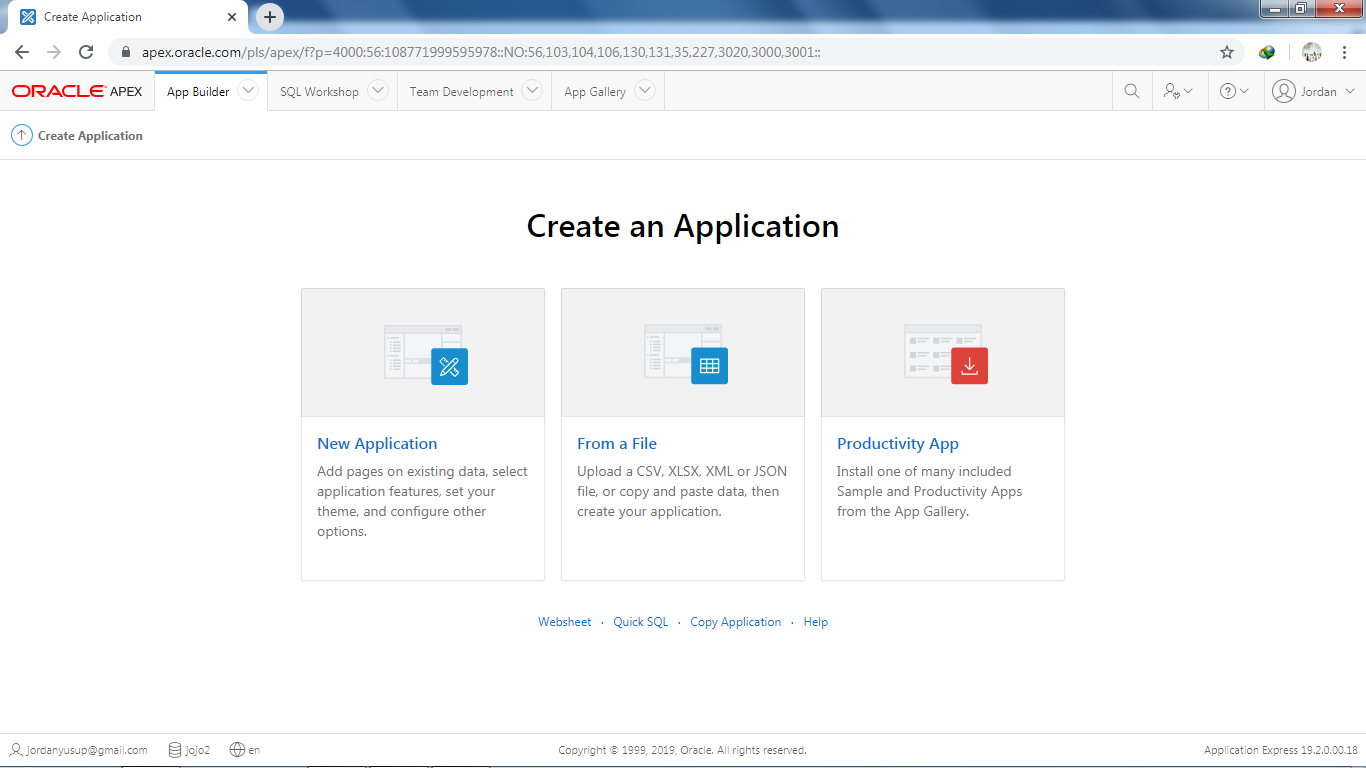
\includegraphics[width=1\textwidth]{figures/2.png}
\end{figure}

\item Kemudian pilih add page
\begin{figure}[H]
\centering
\caption{Add Page}
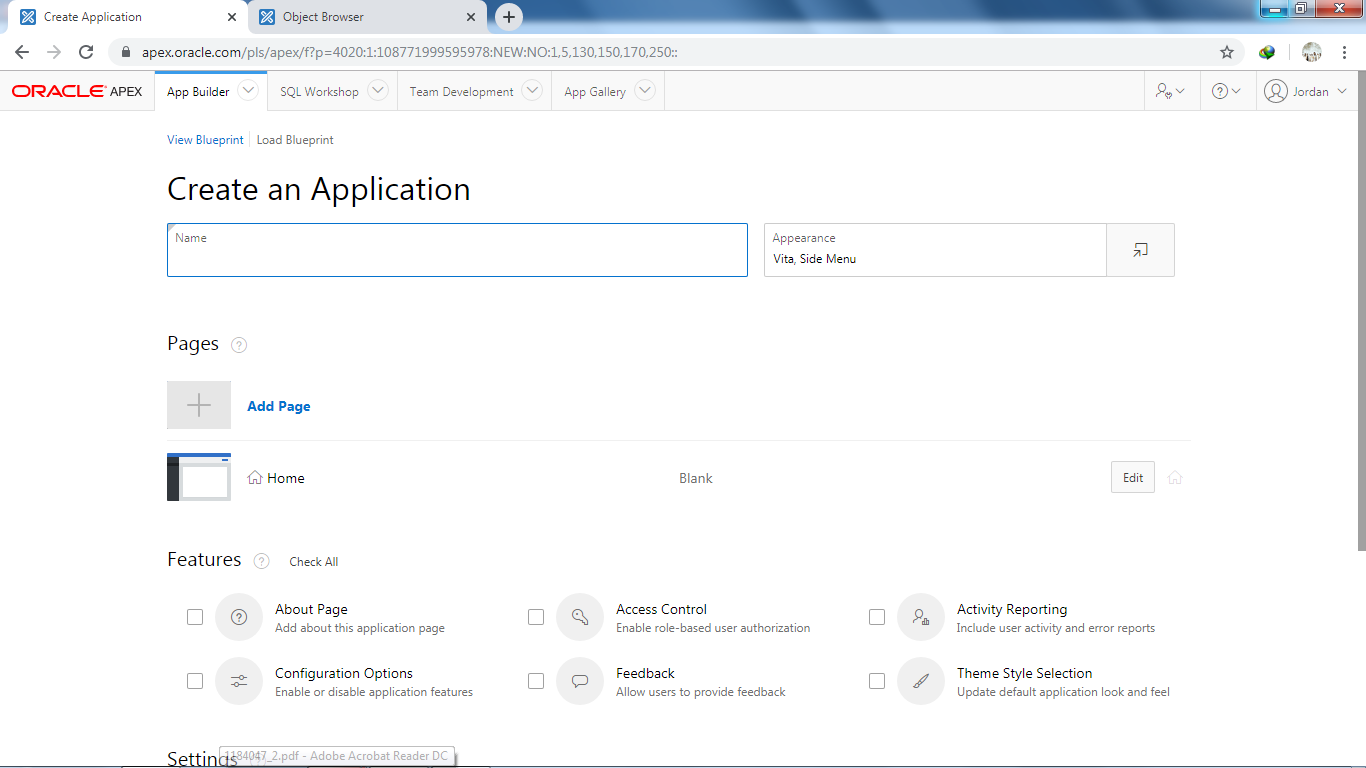
\includegraphics[width=1\textwidth]{figures/14.png}
\end{figure}

\item Pilih interactive report
\begin{figure}[H]
\centering
\caption{Interactive Report}
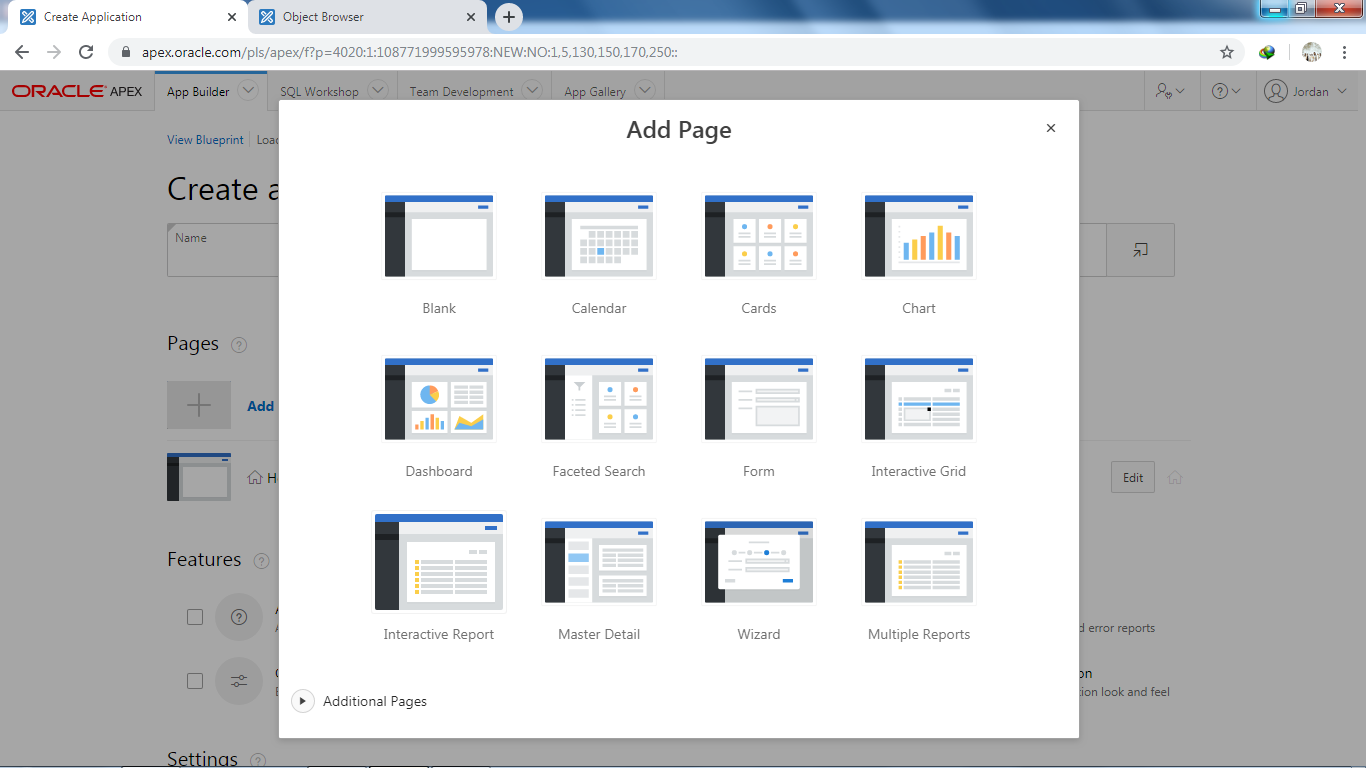
\includegraphics[width=1\textwidth]{figures/15.png}
\end{figure}

\item Klik select table, dan pilih tabelnya
\begin{figure}[H]
\centering
\caption{Pilih Tabel}
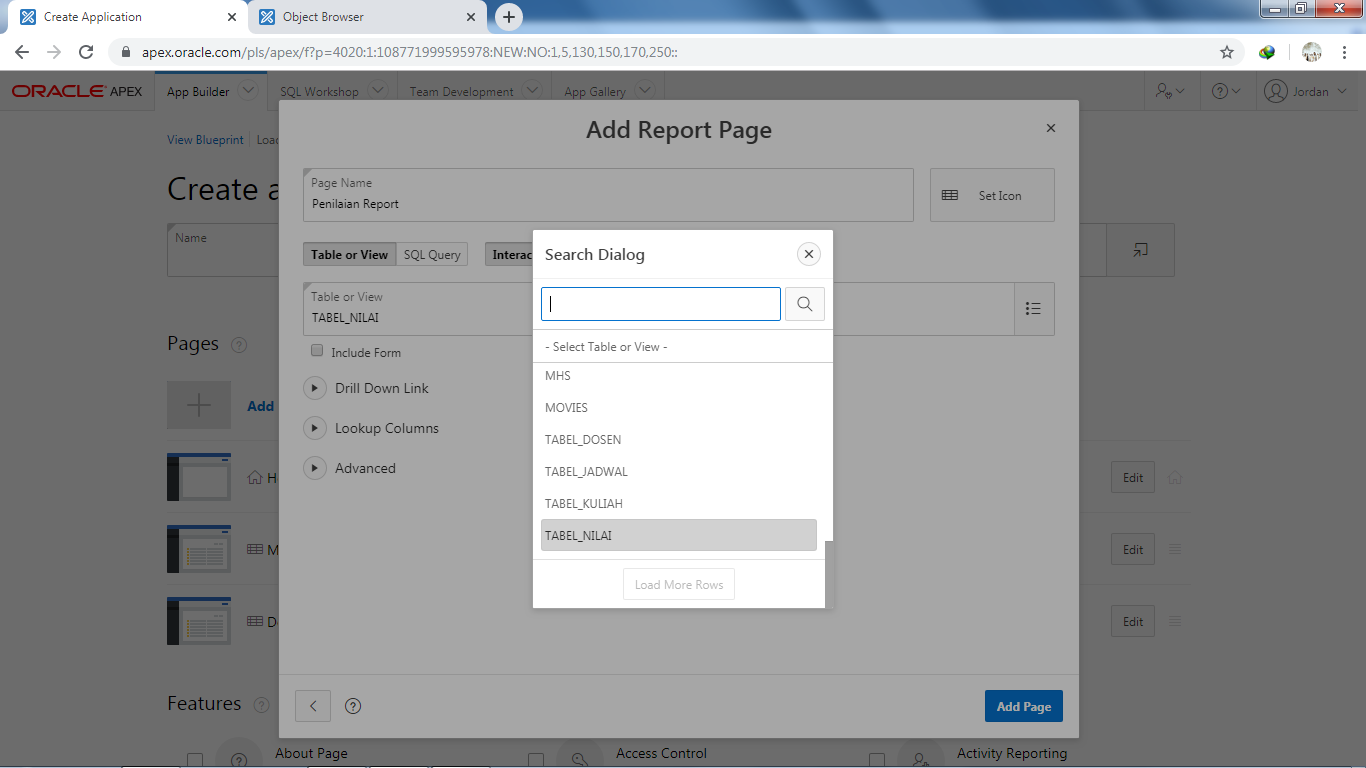
\includegraphics[width=1\textwidth]{figures/16.png}
\end{figure}

\item Kemudian isi page name lalu klik ok
\begin{figure}[H]
\centering
\caption{Isi Page Name}
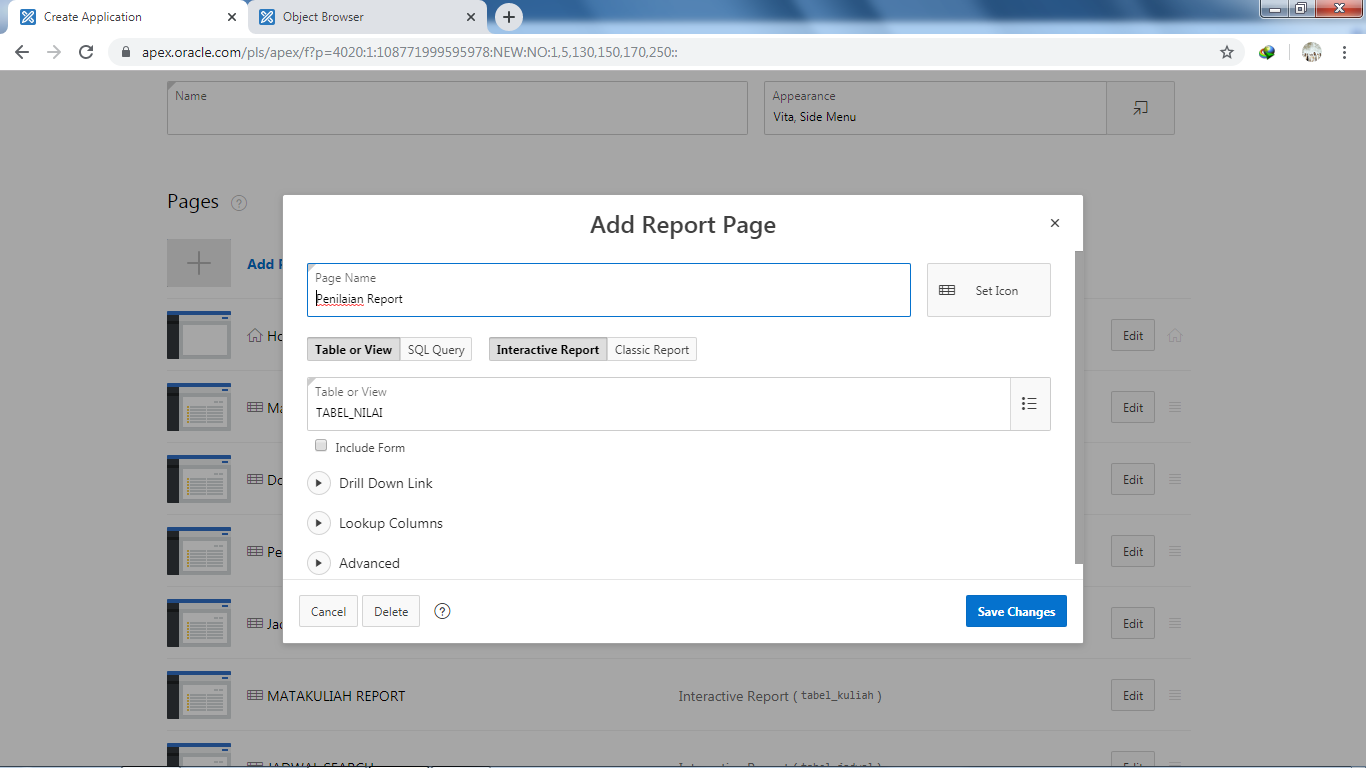
\includegraphics[width=1\textwidth]{figures/17.png}
\end{figure}

\item Ulangi langkah tersebut sesuai kebutuhan.

\item scroll kebawah lalu klik create application

\item Kemudian run application seperti gambar
\begin{figure}[H]
\centering
\caption{Run Application}
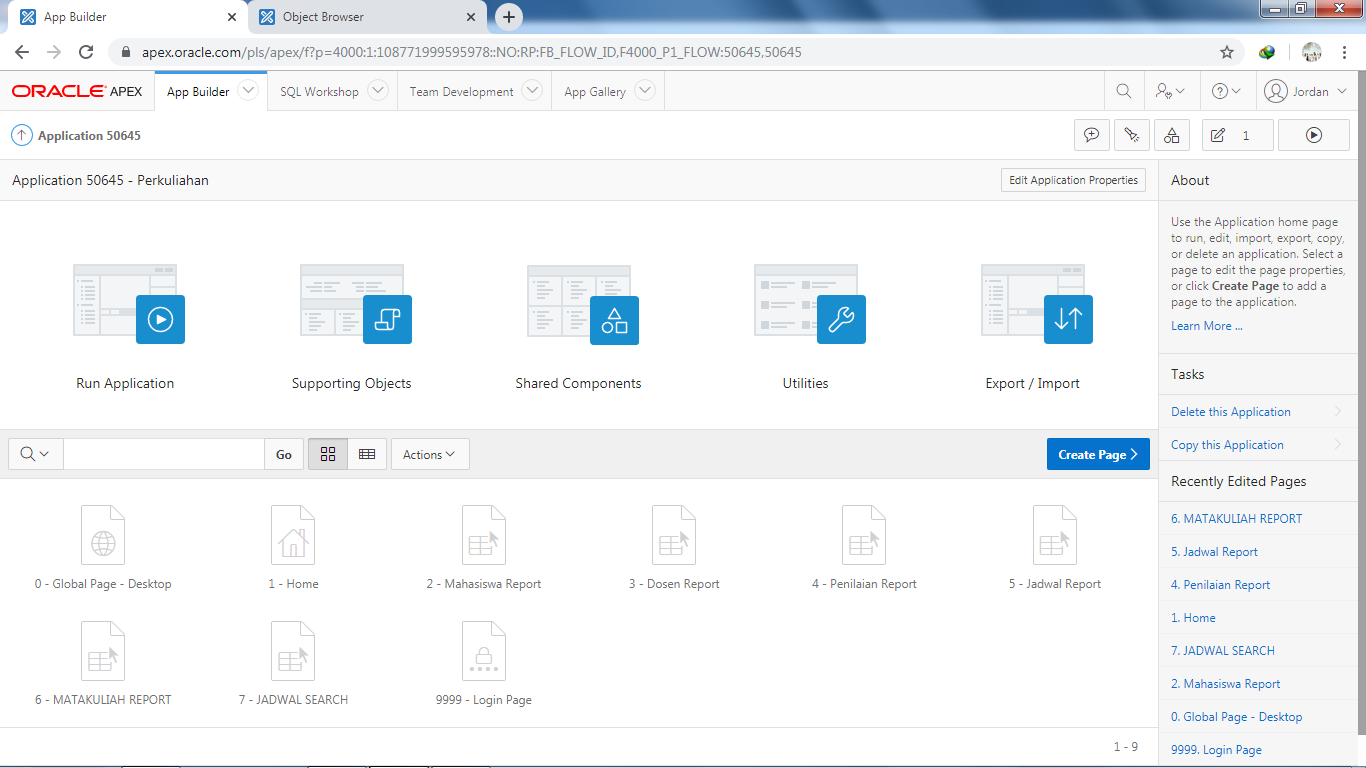
\includegraphics[width=1\textwidth]{figures/18.png}
\end{figure}

\item Hasilnya seperti ini
\begin{figure}[H]
\centering
\caption{Hasil 2}
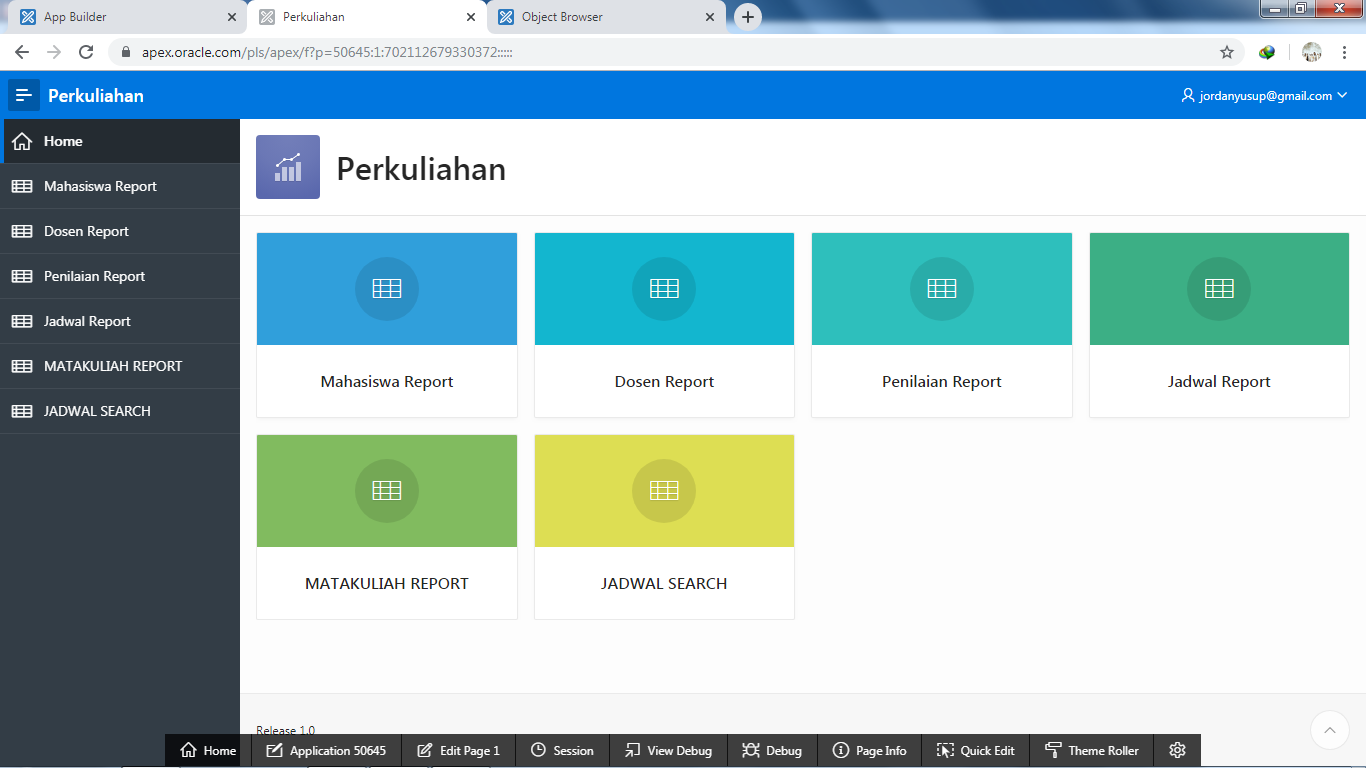
\includegraphics[width=1\textwidth]{figures/19.png}
\end{figure}

\begin{figure}[H]
\centering
\caption{Hasil 2}
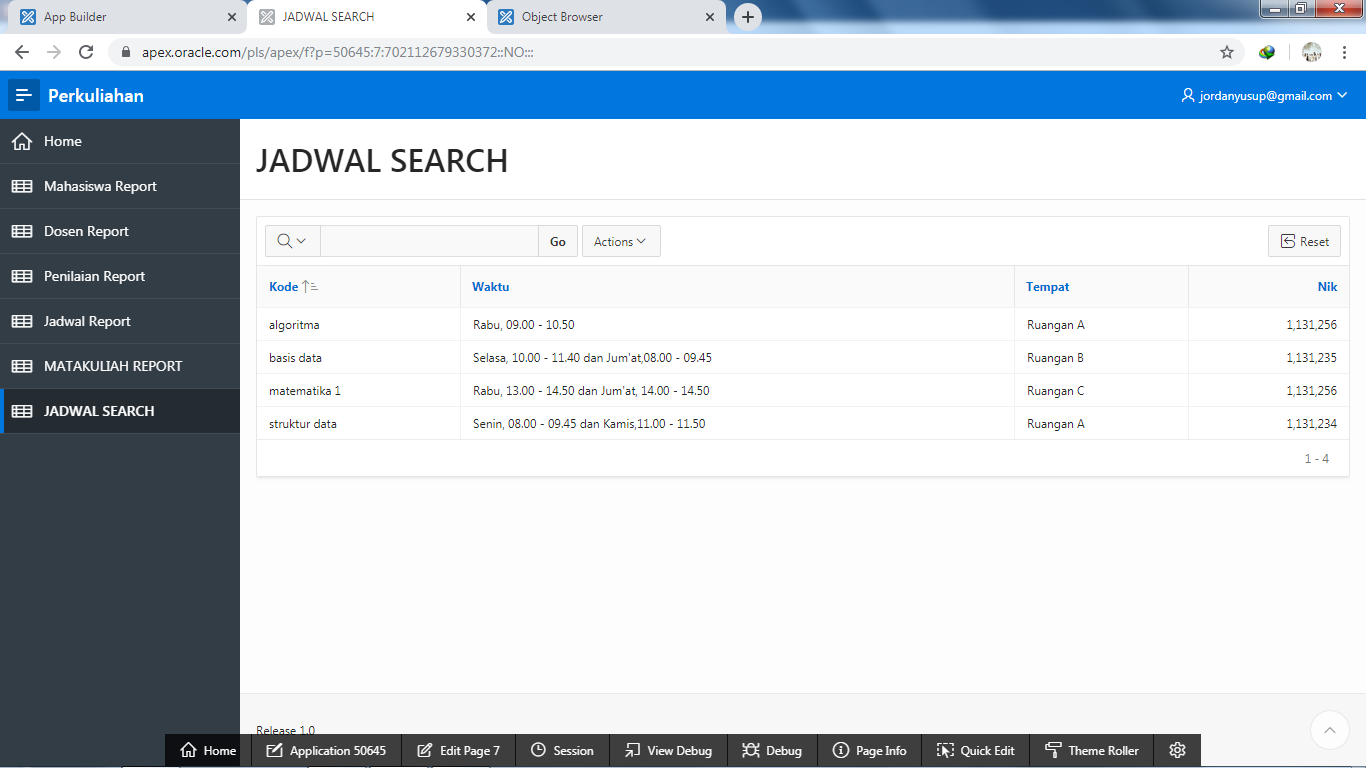
\includegraphics[width=1\textwidth]{figures/20.png}
\end{figure}

\end{enumerate}